% Szglab4
% ===========================================================================
%

\newcommand{\Fn}[3]{

	\SetKwFunction{FMain}{#1}
	\SetKwProg{Fn}{Function}{:}{}
	\Fn{\FMain{#2}}{
		#3
	}
	
	
}
\chapter{Részletes tervek}

\thispagestyle{fancy}

\section{Osztályok és metódusok tervei}

%todo ezt szépíteni
\lstset{
	breakatwhitespace=false,
	breaklines=true,
	tabsize=2,
	frame=L,
	numbers=left,
	basicstyle=\small\ttfamily
}

\section{Osztályok leírása}
\subsection{BareHands}
\begin{itemize}
	\item A játékos így ás, ha nincs ásója. A kiválasztott cellán csökkennie kell a hó mennyiségnek ásáskor.
	\item Interfészek:
	\begin{itemize}
		\item DigStrategy
	\end{itemize}
	\item Metódusok:
	\begin{itemize}
		\item bool Dig(Tile t): Csökkenti a tile-on található hó mennyiségét. Minden alkalommal fárasztó az ásás, ezért a visszatérési érték mindig true.
		\begin{lstlisting}
Decrement Snow amount on t
return true
		\end{lstlisting}
	\end{itemize}
\end{itemize}

\subsection{BareIce}
\begin{itemize}
	\item Ilyen a jégtábla, ha nincs rajta iglu. A jégtáblán nincs védelem a vihar elől.
	\item Ősosztályok:
	\begin{itemize}
		\item Shelter
	\end{itemize}
	\item Metódusok:
	\begin{itemize}
		\item void ChillStorm(Tile t): A paraméterként kapott t Tilen álló játékosok testhője csökken.
		\begin{lstlisting}
for all e : Entity on t
	e gets Chilled
		\end{lstlisting}
		\item void BearAttack(Tile t): A paraméterként kapott t Tilen álló minden játékost megtámad a medve.
		\begin{lstlisting}
for all e : Entity on t
	e gets Attacked by Bear
		\end{lstlisting}
		\item void Break(Tile t): Nem csinál semmit, mert a nem létező menedék nem törik el.
	\end{itemize}
\end{itemize}

\subsection{BuildStrategy}
\begin{itemize}
	\item A játékos így képes építeni. Iglut vagy sátrat.
	\item Attribútumok:
	\begin{itemize}
		\item count: int: Az építhető sátrak számát tárolja.
	\end{itemize}
	\item Metódusok:
	\begin{itemize}
		\item void Build(Tile t): Épít egy sátrat a játékos a paraméterként kapott mezőre. Az építhető sátrak száma eggyel csökken.
		\begin{lstlisting}
if the count of available tents is above 0
	Decrements the amount of available tents.
	Instantiates a Tent object as te
	Sets the shelter of t to te
		\end{lstlisting}
		\item void Gain(): Kap egy sátrat, eggyel nő az építhető átrak száma.
		\begin{lstlisting}
Increments the amount of available tents
		\end{lstlisting}
	
	\end{itemize}
\end{itemize}

\subsection{BreakingShovel}
\begin{itemize}	
	\item Törhető ásó osztály.
	\item Interfészek:
	\begin{itemize}
		\item Item
	\end{itemize}
	\item Metódusok:
	\begin{itemize}
		\item + void GiveTo(Player p): A játékos így kap ásót. Az ásója annyiszor tud majd ásni törés előtt, amennyit ez a metódus beállít neki.
		\begin{lstlisting}
Instantiates a new BreakingShovelDig object as bsd
set the DigStrategy of p to bsd with the durability of the BreakingShovel
		\end{lstlisting}
	\end{itemize}
\end{itemize}

\subsection{BreakingShovelDig}
\begin{itemize}
	\item A játékos így ás, ha törhető ásó van nála.
	\begin{figure}[H]
        \begin{center}
                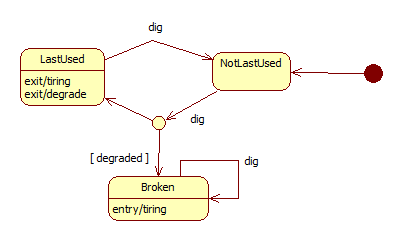
\includegraphics[width=10cm]{chapters/chapter08/BreakingShovelStatechartDiagram.png}
                \caption{BreakingShovelDig StateChart}
                \label{BreakingShovelDig StateChart}
        \end{center}
	\end{figure}
	\item Intefészek:
	\begin{itemize}
		\item DigStrategy
	\end{itemize}
	\item Attribútumok:
	\begin{itemize}
		\item - lastUsed: bool: Volt-e használva a körben.
		\item - durability: int: Mennyiszer lehet még ásni vele.
	\end{itemize}
	\item Metódusok:
	\begin{itemize}
		\item + bool Dig(Tile t): Csökkenti a tile-on található hó mennyiségét.
		\begin{lstlisting}
reduces the durability of this by one
Decrement snow on t
if the item was already used in this turn
	return true
else
	return false
		\end{lstlisting}
	\end{itemize}
\end{itemize}

\subsection{CantRescue}
\begin{itemize}
	\item A játékos nem tudja kihúzni a csapattársát. A játékos ilyen állapotban van, ha nincs nála kötél.
	\item Interfészek:
	\begin{itemize}
		\item RescueStrategy
	\end{itemize}
	\item Metódusok:
	\begin{itemize}
		\item + void Rescue(Tile water, Tile land): Mivel a játékos ebben az állapotban nem tudja megmenteni a csapattársát, ez a fv nem csinál vele semmit. 
	\end{itemize}
\end{itemize}

\subsection{ChillWaterStrategy}
\begin{itemize}
	\item A jégtábla így hűti a vízbe esett játékosokat. Vízben tartózkodás esetén a játékos testhője csökken, a megvalósított stratégia alapján.
	\item Metódusok:
	\begin{itemize}
		\item + abstract void Chill(Tile t): A stratégiát megvalósító elem dolga implementálni mi történik.
	\end{itemize}
\end{itemize}

\subsection{DigStrategy}
\begin{itemize}
	\item A játékos így ás.	Ásáskor a cellán a hómennyiség csökken.
	\item Metódusok:
	\begin{itemize}
		\item + abstract bool Dig(Tile t): A stratégiát megvalósító elem dolga implementálni mi történik ásáskor. Visszaadja, hogy az ásás fárasztó-e.
	\end{itemize}
\end{itemize}

\subsection{DryLand}
\begin{itemize}
	\item A szárazföld nem hűti a játékosokat. A játékos nincsen vízben.
	\item Interfészek:
	\begin{itemize}
		\item ChillWaterStrategy
	\end{itemize}
	\item Metódusok:
	\begin{itemize}
		\item + void Chill(Tile t): A stratégia megvalósítása miatt kér be egy t Tile paramétert, a rajta levő játékossal viszont nem csinál semmit, mert az nincs vízben, nem csökkenti testhőjét.
	\end{itemize}
\end{itemize}

\subsection{Empty}
\begin{itemize}
	\item Nincs jégbe fagyott tárgy. Ez az üres eszköz típus, nem képes semmi extra tulajdonságot biztosítani a tulajdonosnak.
	\item Interfészek:
	\begin{itemize}
		\item Item
	\end{itemize}
	\item Metódusok
	\begin{itemize}
		\item + void GiveTo(Player p): A paraméterként kapott játékost nem ruházza fel extra tulajdonsággal, mivel épp nincs itt jégbe fagyott tárgy.
	\end{itemize}
\end{itemize}

\subsection{Entity}
\begin{itemize}
	\item Entitás osztály ami a pályát tartózkodhat.
	\item Metódusok:
	\begin{itemize}
		\item + Step(int direction): Lép a paraméterként kapott irányba.
		\begin{lstlisting}
Gets the Tile in the dir direction from the current Tile the entity is on
The entity steps off from the Tile
It gets placed on the new Tile
		\end{lstlisting}
		\item + void PlaceOn(Tile t): Ráteszi az entitást egy másik táblára. A kötél használatakor használatos.
		\begin{lstlisting}
The current tile of the entity becomes t
The entity gets placed into the occupants collection of t
		\end{lstlisting}
		\item + void Chill(): Hűti az entitást. A testhője csökken. Nem csinál semmit, csak visszatér, majd a leszármazottak felüldefiniálják.
		\item + void ResistWater(): Így viselkedik vízben. Nem csinál semmit, csak visszatér, majd a leszármazottak felüldefiniálják.
		\item + void BearAttack(): Így viselkedik, ha megtámadja a medve. Nem csinál semmit, csak visszatér, majd a leszármazottak felüldefiniálják.
	\end{itemize}
\end{itemize}

\subsection{Eskimo}
\begin{itemize}
	\item Játékos fajta. 5 egységnyi testhővel kezd. Képes iglut építeni. A játékos irányítja.
	\item Ősosztályok:
	\begin{itemize}
		\item Player
	\end{itemize}
	\item Metódusok:
	\begin{itemize}
		\item + void Build(): Épít egy iglut a mezőre, amin áll, a BuildStrategyjétől függetlenül. Az iglu megvéd majd a hóvihartól. Beállítja a mező menedékét Iglura.
		\begin{lstlisting}
The eskimo's energy decreases by one
An Igloo object is created as i.
The Shelter of the current Tile becomes i
		\end{lstlisting}
	\end{itemize}
\end{itemize}

\subsection{Food}
\begin{itemize}
	\item Élelem, amit a játékos meg tud enni, hogy növelje a testhőjét. Élelem a pályán lesz található.
	\item Interfészek:
	\begin{itemize}
		\item Item
	\end{itemize}
	\item Metódusok:
	\begin{itemize}
		\item + void GiveTo(Player p): A paraméterként kapott játékos kap egy élelmet, az bekerül az élelemtárolójába.
		\begin{lstlisting}
The amount of food in the foodstore of p increases by one
The food is removed from the Player's inventory
		\end{lstlisting}
	\end{itemize}
\end{itemize}

\subsection{FoodStore}
\begin{itemize}
	\item A játékos ebben a zsebben tárolja az élelmet.
	\item Attribútumok:
	\begin{itemize}
		\item - count: int: Hány élelem van a játékosnál.
	\end{itemize}
	\item Metódusok:
	\begin{itemize}
		\item + void feed(Player p): Játékos testhője megnő, az élelem mennyisége csökken, mivel a játékos megeszi azt.
		\begin{lstlisting}
if the foodstore is not empty
The amount of food in the foodstore decreases by one
The body temperature of the player increases by one
		\end{lstlisting}
		\item void Gain(): növeli a benne található elemek számát.
		\begin{lstlisting}
The food count increases by one
		\end{lstlisting}
	\end{itemize}
\end{itemize}

\subsection{Game}
\begin{itemize}
	\item Interface a Model és a Controller között. A játékmesterhez tartozó működést valósítja meg. Felelős a játékban lévő objektumok tárolásáért és létrehozásáért.
	\item Attribútumok:
	\begin{itemize}
		\item - players: Player[3..*]: Tárolja a játékosokat.
		\item - icefield: Tile[1..*]: Tárolja a pályát alkotó elemeket.
		\item - bears: PolarBear[*]: Tárolja a medvé(ke)t, ha több van akkor is.
		\item - subscribers: GameObserver[*]:  Őket értesíti a játék eseményekről.
	\end{itemize}
	\item Metódusok:
	\begin{itemize}
		\item - void AddTile(t: Tile): Hozzáad egy cellát a játékhoz.
		\item - void AddPlayer(pl: Player): Hozzáad egy játékost a játékhoz.
		\item + Tile CreateTile(int: snow, int: weightLimit): Létrehoz egy cellát. 
		\item + Player CreateEskimo(): Létrehoz egy eszkimó játékost.
		\begin{lstlisting}
create default (naked, no items) e : Eskimo;
add e to entities;
return e;
		\end{lstlisting}
		\item + PolarBear CreatePolarBear(): Létrehoz egy medvét.
		\begin{lstlisting}
create b : PolarBear;
add b to entities;
return b;
		\end{lstlisting}		
		\item + Player CreatePolarExplorer(): Létrehoz egy sarkkutató játékost.
		\begin{lstlisting}
create default (naked, no items) p : PolarExplorer;
add p to entities;
return p;		
		\end{lstlisting}
		\item + void Explore(Tile): Szól a feliratkozóknak, hogy egy sarkkutató felderített egy cellát.
		\item + void GameOver(): Ha vége a játéknak, szól a feliratkozóknak, hogy vesztettünk.
		\begin{lstlisting}		
for all observer in observers
	observer.gameOver();
		\end{lstlisting}
		\item + void Subscribe(GameObserver): Belerakja a kollekcióba.
		\item + void Turn(): Ezt a metódust a Controller hívja körönként, a körök vezénylésére szolgál. 
		\begin{lstlisting}
for all p : player in entities {
	p.setEnergy(4);
}
for all t : Tile in tiles {
	t.Chill();
}

if time for snowstorm {
	for all t : Tile in tiles
		t.ChillStorm();
}

for all b: PolarBear in entities
	b.Step();

for all p : player in entities {
	read input for p;
	do turn for p;
}
		\end{lstlisting}
		\item + void Victory(): Ha vége a játéknak, szól a feliratkozóknak, hogy nyertünk.
		\begin{lstlisting}
for all observer in observers
	observer.victory();
		\end{lstlisting}		
		\item + void Unsubscribe(GameObserver): Eltávolítja a kollekcióból.
	\end{itemize}
\end{itemize}

\subsection{GameObserver}
\begin{itemize}
	\item Figyeli a játék eseményeket.
	\item Metódusok:
	\begin{itemize}
		\item + void GameOver(): Vereség esemény.
		\item + void Victory(): Győzelem esemény.
		\item + void Explore(Tile t): Sarkkutató felderít esemény.
	\end{itemize}
\end{itemize}

\subsection{Igloo}
\begin{itemize}
	\item Ezen a jégtáblán iglu áll, a játékosok védve vannak a vihartól. Az ilyen táblán nem csökken a viharban a rajta állók testhője.
	\item Ősosztályok:
	\begin{itemize} 
		\item Shelter
	\end{itemize}
	\item Metódusok:
	\begin{itemize}
		\item + void ChillStorm(Tile t): A paraméterként kapott cellán álló játékosok testhője nem csökken, mivel igluban vannak.
		\item + void BearAttack(Tile t): Így viselkedik a mező ha valaki igluban van és megtámadja a medve. Visszatér, mert a medve az igluban meghúzódó játékosokat nem bántja.
		\item + void Break(): Visszatér, nem csinál semmit, mivel az iglu nem törik el soha.
	\end{itemize}
\end{itemize}

\subsection{Item}
\begin{itemize}
	\item Tárgy, a játékos képes ilyeneket felvenni a cellákról. A tárgyak képesek a játékosak képességeket adni. A tárgyak alapvetően jégbe fagyva vannak a pályán.
	\item Metódusok:
	\begin{itemize}
		\item + void GiveTo(p: Player): A játékos kap valamilyen tárgyat, az Item interfészt megvalósító tárgyak felüldefiniálják ezt.
	\end{itemize}
\end{itemize}

\subsection{Naked}
\begin{itemize}
	\item A játékos védtelen a hideg vízzel szemben. A játékos ha így esik vízbe és nem menekítik ki megfullad.
	\item Interfészek:
	\begin{itemize}
		\item WaterResistanceStrategy
	\end{itemize}
	\item Metódusok:
	\begin{itemize}
		\item + void Chill(Player p): Játékosnak nincsen ereje a vízben úszni búvárruha nélkül.
		\begin{lstlisting}
The energy of p becomes 0.
		p gets Chilled
		\end{lstlisting}
	\end{itemize}
\end{itemize}

\subsection{Part}
\begin{itemize}
	\item Jégbefagyott alkatrész. Csak akkor ásható ki, ha nincs rajta hó.
	\item Interfészek:
	\begin{itemize}
		\item Item
	\end{itemize}
	\item Metódusok:
	\begin{itemize}
		\item + void GiveTo(Player p): A játékos tárolójába kerül egy darab a rakétapisztolyból.
		\begin{lstlisting}
The amount of parts in the partstore of p increases by one
The part is removed from the Player's inventory
		\end{lstlisting}
	\end{itemize}
\end{itemize}

\subsection{PartStore}
\begin{itemize}
	\item A játékos ebben a zsebben tárolja az alkatrészeket.
	\item Attribútumok:
	\begin{itemize}
		\item - count: int: Tárolja hány darab alkatrész van belőle a játékosnál.
	\end{itemize}
	\item Metódusok:
	\begin{itemize}
		\item + void Gain(PartStore ps): Átveszi az alkatrészeket a paraméterként kapott alkatrésztárolóból.
		\begin{lstlisting}
The amount of parts in this store increases by the amount of parts in ps
The amount of parts in ps becomes 0
		\end{lstlisting}
		\item + void Gain(int n): Megnő az alkatrészek száma, ami a játékosnál van.
		\begin{lstlisting}
The amount of parts in the store increases by n
		\end{lstlisting}
		\item + int getCount(): Visszaadja a count aktuális értékét, azaz a rakétadarabok számát.
		\begin{lstlisting}
returns the amount of parts in the store
		\end{lstlisting}
		\item + void setCount(int n): Beállítja a count aktuális értékét a paraméterként kapott rakétadarab számra.
		\begin{lstlisting}
The amount of parts in the store becomes n
		\end{lstlisting}
	\end{itemize}
\end{itemize}

\subsection{Player}
\begin{itemize}
	\item Játékos osztály, amit a felhasználó irányít a grafikus felületen keresztül. Ilyen típussal nem lehet játszani, csak a leszármazottakkal. Felelőssége a játékos által a controlleren keresztül kiadott műveletek elvégzése. Tárolja a játékos jelenlegi állapotát.
	\item Ősosztályok:
	\begin{itemize}
		\item Entity
	\end{itemize}
	\item Attribútumok:
	\begin{itemize}
		\item - bodyTemp: int: Jelzi a játékos jelenlegi hőmérsékletét, ha 0 akkor megfagy $\rightarrow$ játék vége.
		\item - buildStrategy: BuildStrategy: Így tud építeni a játékos.
		\item - currentTile: Tile: A játékos ismeri a mezőt amin éppen áll.
		\item - inventory: Item[*]: Tárolja a játékos tárgyait, amik képességekkel tudjak felruházni őt.
		\item - digStrategy: DigStrategy: Eldönti hogyan képes ásni a játékos.
		\item - energy: int: Számlálja mennyit mozogott az adott körben a játékos.
		\item - foodStore: FoodStore: Tárolja a játékos ételeit.
		\item - game: Game: A játékos ismeri a játékot.
		\item - partStore: PartStore: Tárolja a játékos rakéta alkatrészeit.
		\item - rescueStrategy: RescueStrategy: Eldönti, hogy megmenthet egy játékos egy másikat a vízbeesés után.
		\item - waterResistanceStrategy: WaterResistanceStrategy: Eldönti, hogy a játékos hogyan viselkedik vízbeesés esetén.
	\end{itemize}
	\item Metódusok:
	\begin{itemize}
		\item + void AssembleFlare(): Összerakja a játék végéhez szükséges rakéta pisztolyt. 1 munkaegység\\
		\begin{algorithm}[H]
			\Fn{AssembleFlare}{}{
				\If{Every player is on the same tile \textbf{and} The players have three FlareParts} {
					Victory
				}
			}
		\end{algorithm}
		\item + void Build(): A játékos épít.\\
		\begin{algorithm}[H]
			\Fn{Build}{}{
				decrement energy \\
				buildStrategy.Build(currentTile)
			}
		\end{algorithm}
		\item + void BearAttack(): A játékost medvetámadás éri.\\
		\begin{algorithm}[H]
			\Fn{BearAttack}{}{
				Game Over
			}
		\end{algorithm}
		\item + void Chill(): A testhő 1-el csökken, ha 0 alá megy $\rightarrow$ GameOver.\\
		\begin{algorithm}[H]
			\Fn{Chill}{}{
				Decrements body temperature \\ 
				\If {body temp equals to 0} {
					The game is over
				}
			}
		\end{algorithm}
		\item + void DecrementEnergy(): Az energiát csökkentő helper metódus.\\
		\begin{algorithm}[H]
			\Fn{decrementEnergy}{}{
				Decrements the energy of the player
			}
			
		\end{algorithm}
		\item + void Dig(): Ezt a metódust a Controller hívja. A játékos havat ás. 1 munkaegység\\
		\begin{algorithm}[H]
			\Fn{Dig}{}{
				\If{Energy is greater than 0} {
					Decrement energy \\
					Dig based on the player's digStrategy
				}
			}
		\end{algorithm}
		\item + void EatFood(): Ezt a metódust a Controller hívja. A játékos eszik. A testhője megnő 1-el.\\
		\begin{algorithm}[H]
			\Fn{EatFood}{}{
				Try to eat food from the FoodStore
			}
		\end{algorithm}
		\item + void PickUp(): Ezt a metódust a Controller hívja. A játékos felvesz egy tárgyat. 1 munkaegység\\
		\begin{algorithm}[H]
			\Fn{pickUp}{}{
				\If {Energy is greater than 0}{
					Decrement energy \\
					Move the item from the current tile to the inventory of the player
				}	
			}	
		\end{algorithm}
		\item + void Equip(inventorySlot: int): Ezt a metódust a Controller hívja. A játékos kiválaszt egy tárgyat használatra.\\
		\begin{algorithm}[H]
			\Fn{Equip}{int inventorySlot}{
				Make the item in the inventorySlot-th slot active
			}
		\end{algorithm}
		%\item + void PlaceOn(Tile t): Init szekvencia része. RopeRescue szekvencia része. Rárak egy játékost egy másik Tile-ra.\\
		%\begin{algorithm}[H]
		%	\Fn{placeOn}{Tile t}{
		%		Place the player on tile t
		%	}
		%\end{algorithm}
		\item + void RescueTeammate(direction: int): Ezt a metódust a Controller hívja. A játékos kiment egy másikat a vízből. 1 munkaegység\\
		\begin{algorithm}[H]
			\Fn{RescueTeammate}{int d}{
				\If{Energy is greater than 0} {
					Decrement energy \\
					Try to rescue the teammate on the neighbor tile in direction d based on the player's rescueStrategy
				}
			}
		\end{algorithm}
		\item + void ResistWater(): A játékos testhője a WaterResistance szerint változik.\\
		\begin{algorithm}[H]
			\Fn{ResistWater}{}{
				Resist water based on the player's waterResistanceStrategy
			}
		\end{algorithm}
		\item + void Step(direction: int): Ezt a metódust a Controller hívja. A játékos lép, ha van még hozzá elég energiája. 1 munkaegység\\
		\begin{algorithm}[H]
			\Fn{Step}{int direction}{
				\If{Energy is greater than 0} {
					Decrement energy \\
					Move the player to the next tile in the given direction
				}
			}
		\end{algorithm}
		\item + void ToFoodStore(): Élelem megtalálásához helper metódus.
	\end{itemize}
\end{itemize}

\subsection{PolarBear}
\begin{itemize}
	\item Jegesmedve osztály. Random lépeget a táblán és ha playert talál megtámadja azt.
	\item Ősosztályok:
	\begin{itemize}
		\item Entity
	\end{itemize}
	\item Metódusok:
	\begin{itemize}
		\item + void Step(int direction): Lép az adott irányba.
		\begin{lstlisting}
Calls the Step method of base class with parameter direction
Attacks the tile it has stepped on
		\end{lstlisting}
		\item + void Chill(): Nem csinál semmit, csak visszatér, mert a jegesmaci nem fázik.
		\item + void ResistWater(): Nem csinál semmit, csak visszatér, mert a jegesmaci a vízben sem fázik.
		\item void BearAttack(): Nem csinál semmit, csak visszatér, mert a jegesmaci nem támadja meg fajtársait, kizárólag a játékos húsát ízleli örömmel.
		\item + void PlaceOn(Tile t): A medve átkerül a paraméterként kapott t Tilera.
		\begin{lstlisting}
The current tile of the polar bear becomes t.
The bear gets placed into the occupants collection of t.
		\end{lstlisting}
	\end{itemize}
\end{itemize}

\subsection{PolarExplorer}
\begin{itemize}
	\item Játékos fajta. 4 egységnyi testhővel kezd. Képes megnézni egy cella teherbíró képességét. A játékos irányítja.
	\item Ősosztályok:
	\begin{itemize}
		\item Player
	\end{itemize}
	\item Metódusok:
	\begin{itemize}
		\item + void Examine(dir: int): A játékos megnézheti, hogy egy adott irányban lévő Tile-nak mennyi a teherbírása. A Game.Explore metódust hívja.
		\begin{lstlisting}
Gets the tile in the dir direction from the current tile he is on, calls it t
Calls the Explore method of the game objects he knows of with the t as a parameter.
		\end{lstlisting}
	\end{itemize}
\end{itemize}

\subsection{RescueStrategy}
\begin{itemize}
	\item A játékos így húzza ki csapattársát a vízből. A játékos így képes megmenteni a vízbe esett csapattársát a szomszédos celláról, a megvalósított stratégia alapján. Kötél szükséges a másik játékos megmentéséhez.
	\item Metódusok:
	\begin{itemize}
		\item + abstract void Rescue(Tile water, Tile land): A stratégiát megvalósító elem dolga implementálni mi történik.
	\end{itemize}
\end{itemize}

\subsection{Rope}
\begin{itemize}
	\item Jégbe fagyott kötél. Ezzel lehet megmenteni a vízbe esett csapattársat a szomszédos celláról.
	\item Interfészek:
	\begin{itemize}
		\item Item
	\end{itemize}
	\item Metódusok
	\begin{itemize}
		\item + void GiveTo(Player p): A játékos kap egy kötelet. Az bekerül az inventoryjába és a megfelelő stratégiájához is a kötél által adott képesség.
		\begin{lstlisting}
Instantiates a RopeRescue object as rr
Sets the RescueStrategy of p to rr
		\end{lstlisting}
	\end{itemize}
\end{itemize}

\subsection{RopeRescue}
\begin{itemize}
	\item A játékos kihúzza csapattársát a vízből. A játékos így menti meg a szomszédos cellán vízbe esett csapattársát.
	\item Interfészek:
	\begin{itemize}
		\item RescueStrategy
	\end{itemize}
	\item Metódusok:
	\begin{itemize}
		\item + void Rescue(Tile water, Tile land): A vízben lévők közül egyvalaki rákerül a kihúzó játékos cellájára.
		\begin{lstlisting}
Asks for the collection of occupants in the water Tile
If there are more than 0 occupants
	The first occupant in the collection gets placed on the land Tile
	That occupant also steps off the water
		\end{lstlisting}
	\end{itemize}
\end{itemize}

\subsection{ScubaGear}
\begin{itemize}
	\item Jégbe fagyott búvárruha. Ezzel lehet életben maradni a vízben.
	\item Interfészek:
	\begin{itemize}
		\item Item
	\end{itemize}
	\item Metódusok:
	\begin{itemize}
		\item + void GiveTo(): A játékos búvárruhát kap. Az bekerül az inventoryjába és a megfelelő stratégiája helyére is a búvárruha által adott képesség.
		\begin{lstlisting}
Instantiates a ScubaWearing object as sw
Sets the WaterResistanceStrategy of p to sw
		\end{lstlisting}
	\end{itemize}
\end{itemize}

\subsection{ScubaWearing}
\begin{itemize}
	\item A játékos testhője nem csökken a vízben. A játékos nem hal bele, ha a vízben marad.
	\item Interfészek:
	\begin{itemize}
		\item WaterResistanceStrategy
	\end{itemize}
	\item Metódusok:
	\begin{itemize}
		\item + void Chill(p: Player): A játékost nem hűti a víz, mivel búvárruhát visel. A metódus csak visszatér, nem csinál semmit.
	\end{itemize}
\end{itemize}

\subsection{Sea}
\begin{itemize}
	\item Ez a cella tenger, hűti a játékosokat.
	\item Interfészek:
	\begin{itemize}
		\item ChillWaterStrategy
	\end{itemize}
	\item Metódusok:
	\begin{itemize}
		\item + void Chill(Tile t): Minden rajta álló testhője csökken a WaterResistanceStrategy szerint.
		\begin{lstlisting}
For all e : Entities on Tile t
	e tries to ResistWater
		\end{lstlisting}
	\end{itemize}
\end{itemize}

\subsection{Shelter}
\begin{itemize}
	\item Ez az absztrakt osztály a menedéket jelképezi egy mezőn.
	\item Metódusok:
	\begin{itemize}
		\item + void ChillStorm(Tile t): Minden a paraméterként kapott t mezőn lévő entitás fázik.
		\begin{lstlisting}
For all e : Entities on t
	e gets Chilled.
		\end{lstlisting}
		\item + void BearAttack(Tile t): A menedéken lévő játékosok medvetámadás áldozatai lesznek.
		\begin{lstlisting}
For all e : Entities on t
	e gets Attacked by bear
		\end{lstlisting}
		\item + void Break(Tile t): Az adott mezőn lévő menedék eltörik. Nem csinál semmit, majd a különböző menedéktípusok másképp definiálják felül.
	\end{itemize}
\end{itemize}

\subsection{Shovel}
\begin{itemize}
	\item Jégbe fagyott ásó. Ezzel lehet több havat eltakarítani a celláról.
	\item Interfészek:
	\begin{itemize}
		\item Item
	\end{itemize}
	\item Metódusok:
	\begin{itemize}
		\item + void GiveTo(): A játékos ásót kap, ami bekerül az inventoryjába és a megfelelő stratégiájához is bekerül az ásó által adott képesség.
		\begin{lstlisting}
Instantiates a ShovelDig object as sd
Sets the DigStrategy of p to sd
		\end{lstlisting}
	\end{itemize}
\end{itemize}

\subsection{ShovelDig}
\begin{itemize}
	\item Egyszer lehet ásni vele fáradság nélkül is.
	\begin{figure}[H]
        \begin{center}
                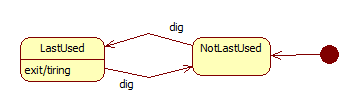
\includegraphics[width=10cm]{chapters/chapter08/ShovelStatechartDiagram.png}
                \caption{ShovelDig StateChart}
                \label{ShovelDig StateChart}
        \end{center}
	\end{figure}
	\item Interfészek:
	\begin{itemize}
		\item DigStrategy
	\end{itemize}
	\item Attribútumok:
	\begin{itemize}
		\item - lastUsed: bool: Volt-e már használva a körben.
	\end{itemize}
	\item Metódusok:
	\begin{itemize}
		\item + bool Dig(Tile t): Csökkenti a tile-on található hó mennyiségét. Minden második alkalommal fárasztó.
		\begin{lstlisting}
Decrements the snow amount on t
if it was already used this turn
	return true
else 
	return false
		\end{lstlisting}
	\end{itemize}
\end{itemize}

\subsection{Tent}
\begin{itemize}
	\item Sátor osztály. Le lehet rakni táblára.
	\item Ősosztályok:
	\begin{itemize}
		\item Shelter
	\end{itemize}
	\item Metódusok:
	\begin{itemize}
		\item + void ChillStorm(Tile t): Így viselkedik a tábla, ha sátor van rajta hóviharban. A sátorban lévő játékosok nem fáznak, a metódus csak visszatér, nem csinál semmit.
		\item + void Break(Tile t): Így viselkedik a sátor, ha eltörik. Beállítja a paraméterként kapott Tile menedékét sima jégre, ezzel jelezve halálát.
		\begin{lstlisting}
sets the Shelter of t to BareIce
		\end{lstlisting}
	\end{itemize}
\end{itemize}

\subsection{TentKit}
\begin{itemize}
	\item Sátor építését lehetővé teszi.
	\item Interfészek:
	\begin{itemize}
		\item Item
	\end{itemize}
	\item Metódusok:
	\begin{itemize}
		\item + void GiveTo(Player p): A játékos így kap sátor alapanyagot.
		\begin{lstlisting}
The BuildStrategy of p Gains a charge.
Removes the Tent from the inventory of p
		\end{lstlisting}
	\end{itemize}
\end{itemize}

\subsection{Tile}
\begin{itemize}
	\item Cella, ilyenekből áll a jégmező ahol a játékosok játszanak.
	\item Attribútumok:
	\begin{itemize}
		\item - chillStormStrategy: ChillStormStrategy: Eldönti, kinek változik a testhője vihar esetén.
		\item - chillWaterStrategy: ChillWaterStrategy: Eldönti, kinek változik a testhője víz esetén.
		\item - item: Item: Ezt a tárgyat lehet kiásni belőle.
		\item - neighborTiles: Tile[*]: Szomszédos cellákat ismer.
		\item - occupants: Entity[*]: Rajta lévő entitások.
		\item - snow: int: Rajta lévő hómennyiség.
		\item - weightLimit: int: Rajta lévő játékosok számának maximuma.		
	\end{itemize}
	\item Metódusok:
	\begin{itemize}
		\item - void Add(Entity): Hozzáad egy entitást a táblához.
		\item + void BreakShelter(): Ez a metódus eltávolítja a sátrat a tábláról.
		\begin{lstlisting}
Calls the break method of the current shelter
		\end{lstlisting}
		\item + void BearAttack(): Medve megtámadja a cellán állókat.
		\item + void ChillStorm(): Ezt a metódust a Controller hívja viharban. Hűti a játékosokat, ha nincsenek igluban vagy sátorban.
		\item + void ChillWater(): Ezt a metódust a Controller hívja körönként. Hűti a játékosokat, ha ez a cella víz.
		\item + void DecrementSnow(): A hómennyiséget csökkentő helper függvény.
		\begin{lstlisting}
if ( snow > 0 )
	decrement snow
		\end{lstlisting}
		\item - void Remove(Entity): Eltávolítja a rajta álló entitást.
		\item + Item TakeItem(): A játékos megkapja a tartalmazott tárgyat.
		\begin{lstlisting}
if( Tile has item on it)
	Remove item from the tile
	return the item
		\end{lstlisting}
		\item + Tile NeighborAt(direction): Visszaadja az adott irányban szomszédos cellát.
		\begin{lstlisting}
return neighbor tile at direction
		\end{lstlisting}
		\item + StepOn(Entity): Játékos rálép a cellára, ha többen vannak mint a korlát, a jégtábla átfordul. A függvény futása során beállítja a megfelelő adattagokat az új értékekre.
		\begin{lstlisting}
Add player to the tile
if ( weight limit is exceeded ) {
	Set tile to sea
	Chill the occupying players on the tile
}
		\end{lstlisting}
		\item + StepOff(Entity): Játékos lelép a celláról. A függvény futása során beállítja a megfelelő adattagokat az új értékekre.
		\begin{lstlisting}
if ( player is on the tile )
	remove player
		\end{lstlisting}
	\end{itemize}
\end{itemize}

\subsection{WaterResistanceStrategy}
\begin{itemize}
	\item Így reagál a játékos a hideg vízre. A vízben búvárruha nélkül nem lehet mozogni. A vízből ha búvárruha nélkül nem húznak ki, nem lehet életben maradni.
	\item Metódusok:
	\begin{itemize}
		\item + abstract void Chill(Player p): A stratégiát megvalósító elem dolga implementálni mi történik.
	\end{itemize}
\end{itemize}

\subsection{Proto}
\begin{itemize}
\item Felelősség\newline
Beolvas parancsokat, értelmezi és futtatja őket.
\begin{figure}[H]
	\begin{center}
			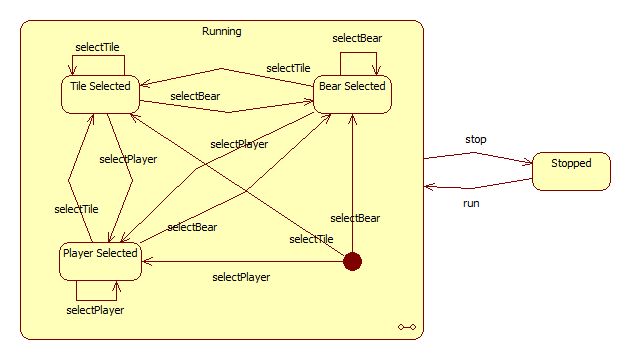
\includegraphics[width=14cm]{chapters/chapter08/ProtoStatechartDiagram.png}
			\caption{Proto StateChart}
			\label{Proto StateChart}
	\end{center}
\end{figure}
\item Attribútumok
	\begin{itemize}
		\item \texttt{+game: Game}; \newline
		A teljes játékot tartalmazza.
		\item \texttt{-running: boolean;} \newline
		A parancsok feldolgozása megállítható vele.
		\item \texttt{-parsers: CommandParser[*];} \newline
		Ilyen parancsokat tud feldolgozni.
		\item \texttt{-selectedTile: Tile[0..1];}
		\item \texttt{-selectedPlayer: Player[0..1];}
		\item \texttt{-selectedBear: PolarBear[0..1];}
		\item \texttt{+selectTile(Tile t);} \newline			
		Beállítja a selectedTile-t és lenullozza a selectedPlayert és a selectedBeart.			
		\item \texttt{+selectPlayer(Player t);} \newline
		Beállítja a selectedPlayer-t és lenullozza a selectedTile-t és a selectedBeart.	
		\item \texttt{+selectBear(PolarBear t);} \newline			
		Beállítja a selectedBeart és lenullozza a selectedTile-t és a selectedPlayert.			
		\item \texttt{+hasSelectedTile(): boolean;}
		\item \texttt{+hasSelectedPlayer(): boolean;}
		\item \texttt{+hasSelectedBear(): boolean;}
		\item \texttt{+getSelectedTile(): Tile;} \newline
		Kivételt dob ha nincs kiválaszvta dolog.			
		\item \texttt{+getSelectedPlayer(): Player;} \newline
		Kivételt dob ha nincs kiválaszvta dolog.
		\item \texttt{+getSelectedBear(): PolarBear;} \newline
		Kivételt dob ha nincs kiválaszvta dolog.
	\end{itemize}
\item Metódusok
	\begin{itemize}
		\item \texttt{+Proto();}
		\begin{lstlisting}
create game;
create MessagePrinter(this);
game.subscribe(the message printer);
createParsers();
		\end{lstlisting}
		\item \texttt{-createParsers();} \newline			
		Készít egy-egy példányt a beépített CommandParserekből és feltölti velük a parsers kollekciót.
		\item \texttt{+run();} \newline
		Fut a parancsértelmezés.
		\begin{lstlisting}
running = true;
while (running) {
	getCommand();
	try {
		command.execute(this);
	} catch (an exception that we threw) {
		print a meaningful error message;
	}
}	
		\end{lstlisting}	
		\item \texttt{+stop();} \newline
		Megáll a parancsértelmezés. A running változó false lesz.
		\item \texttt{-getCommand(): Command;} \newline
		Beolvas egy parancsot a standard bemenetről.
		\begin{lstlisting}
while (true) {
	read line;
	strip comments and trailing whitespace;
	tokenize by spaces;
	if (there are tokens) {
		the first token is the keyword;
		find CommandParser by keyword;
		if (not found) print a meaningful error message;
		else return CommandParser.parse(tokens);
	}
}
		\end{lstlisting}	
		\end{itemize}
\end{itemize}

\subsection{MessagePrinter}
\begin{itemize}
\item Felelősség\newline
Kiírja a konzolra a játék eseményeket.
\item Interfészek\newline
GameObserver
\item Attribútumok
	\begin{itemize}
		\item \texttt{-proto: Proto;}
	\end{itemize}
\item Metódusok
\begin{itemize}
		\item \texttt{+MessagePrinter(proto: Proto);}
		\item \texttt{+victory();} \newline
		Győzelem üzenet kiírása, aztán proto.stop().
		\item \texttt{+gameOver();} \newline
		Vereség üzenet kiírása, aztán proto.stop().
		\item \texttt{+explore(Tile);} \newline
		Tile.weightLimit kiírása.		
	\end{itemize}
\end{itemize}

\subsection{Command}
\begin{itemize}
\item Felelősség\newline
Parancs, végrehajtható formában.
\item Metódusok
\begin{itemize}
		\item \texttt{+execute(state: Proto): abstract void;} \newline
		Végrehajtás az adott állapoton.
		\item \texttt{+toString(): abstract String;} \newline
		Így jelenik meg a konzolon.
	\end{itemize}
\end{itemize}

\subsection{CommandParser}
\begin{itemize}
\item Felelősség\newline
Elkészít egy fajta parancsot.
\item Attribútumok
	\begin{itemize}
		\item \texttt{+/keyword: abstract String \string{readOnly\string};} \newline
		A parancs kulcsszava.
	\end{itemize}
\item Metódusok
\begin{itemize}
		\item \texttt{+parse(tokens: String[1..*] \string{seq\string}): abstract Command;} \newline
		 Parancs elkészítése tokenekből.
	\end{itemize}
\end{itemize}

\subsection{TileCommand}
\begin{itemize}
\item Felelősség\newline
Cella definíciós parancs.
\item Interfészek\newline
Command
\item Metódusok
\begin{itemize}
		\item \texttt{+toString(): String;}
		\begin{lstlisting}
return "tile " + snow + " " + weightLimit;
		\end{lstlisting}
		\item \texttt{+execute(state: Proto);} \newline
		Készít egy Tile-t Game.createTile használatával, majd kiválasztja proto.selectTile-el.
	\end{itemize}
\end{itemize}
\subsection{TileCommandParser}
\begin{itemize}
\item Interfészek\newline
CommandParser
\item Attribútumok
	\begin{itemize}
		\item \texttt{+/keyword: String = "tile";}
	\end{itemize}
\item Metódusok
\begin{itemize}
		\item \texttt{+parse(tokens: String[1..*] \string{seq\string}): Command;}
		\begin{lstlisting}
snow is the second token as a decimal integer;
if (the thid token equals "*") weightLimit is 999;
else weightLimit is the third token as a decimal integer;
create TileCommand;
		\end{lstlisting}
	\end{itemize}
\end{itemize}

\subsection{BuildingCommand}
\begin{itemize}
\item Felelősség\newline
Épület (Iglu vagy Sátor) definíciós parancs.
\item Interfészek\newline
Command
\item Metódusok
\item Attribútumok
	\begin{itemize}
		\item \texttt{-type: String;}
	\end{itemize}
\begin{itemize}
		\item \texttt{+BuildingCommand(type: String);}
		\item \texttt{+toString(): String;}
		\begin{lstlisting}
return "building " + type;
		\end{lstlisting}
		\item \texttt{+execute(state: Proto);}
		\begin{lstlisting}
if (type equals "igloo") create Igloo;
if (type equals "tent") create Tent;
set state.selectedTile.shelter;
		\end{lstlisting}
	\end{itemize}
\end{itemize}
\subsection{BuildingCommandParser}
\begin{itemize}
\item Interfészek\newline
CommandParser
\item Attribútumok
	\begin{itemize}
		\item \texttt{+/keyword: String = "building";}
	\end{itemize}
\item Metódusok
\begin{itemize}
		\item \texttt{+parse(tokens: String[1..*] \string{seq\string}): Command;}
		\begin{lstlisting}
the second token is the type;
accept only "igloo" or "tent";
create BuildingCommand;
		\end{lstlisting}
	\end{itemize}
\end{itemize}

\subsection{ItemCommand}
\begin{itemize}
\item Felelősség\newline
Tárgy definíciós parancs.
\item Interfészek\newline
Command
\item Metódusok
\item Attribútumok
	\begin{itemize}
		\item \texttt{-type: String;}
		\item \texttt{+count: int = 1;}
		\item \texttt{+durability: int = -1;}	
	\end{itemize}
\begin{itemize}
		\item \texttt{+ItemCommand(type: String);}
		\item \texttt{+toString(): String;}
		\begin{lstlisting}
if (count > 1) {
	if (type equals "shovel" and durability > -1)
		return "item shovel " + count + " durability " + durability; 
	else 
		return "item " + type + " " + count;
}
else {
	if (type equals "shovel" and durability > -1)
		return "item shovel durability " + durability; 
	else 
		return "item " + type;
}
		\end{lstlisting}
		\item \texttt{+execute(state: Proto);}
		\begin{lstlisting}
if (state has tile selected and count > 1)
	throw an exception;
if (state has no tile selected and state has no player selected)
	throw an exception;
for (count times) {
	if (type equal "empty") create Empty;
	if (type equal "food") create Food;
	if (type equal "part") create Part;
	if (type equal "scubagear") create ScubaGear;
	if (type equal "rope") create Rope;
	if (type equal "tentkit") create TentKit;
	if (type equal "shovel") {
		if (durability > -1) create BreakingShovel with durability;
		else create Shovel;
	}
	if (state has tile selected)
		set state.selectedTile.item;
	if (state has player selected)
		add item to player inventory;
}	
		\end{lstlisting}
	\end{itemize}
\end{itemize}
\subsection{ItemCommandParser}
\begin{itemize}
\item Interfészek\newline
CommandParser
\item Attribútumok
	\begin{itemize}
		\item \texttt{+/keyword: String = "item";}
	\end{itemize}
\item Metódusok
\begin{itemize}
		\item \texttt{+parse(tokens: String[1..*] \string{seq\string}): Command;}
		\begin{lstlisting}
the second token is the type;
accept only "empty", "food", "part", "scubagear", "rope", "tentkit", "shovel"
create ItemCommand with type;
if (type equals "shovel") {
	if (the third token equals "durability") {
		the fourth token is the durability as a decimal integer;
		set the ItemCommand.durability;
	}
	else {
		the third token is the count as a decimal integer;
		set the ItemCommand.count;
		if (the fourth token equals "durability") {
			the fifth token is the durability as a decimal integer;
			set the ItemCommand.durability;
		}
	}
}
else {
	the third token is the count as a decimal integer;
	set the ItemCommand.count;
}
return the ItemCommand;
		\end{lstlisting}
	\end{itemize}
\end{itemize}

\subsection{EquipCommand}
\begin{itemize}
\item Felelősség\newline
Tárgy kiválasztó parancs.
\item Interfészek\newline
Command
\item Metódusok
\item Attribútumok
	\begin{itemize}
		\item \texttt{-index: int;}
	\end{itemize}
\begin{itemize}
		\item \texttt{+EquipCommand(index: int);}
		\item \texttt{+EquipCommand();} \newline
		"equip all" parancs. Az index -1;
		\item \texttt{+toString(): String;}
		\begin{lstlisting}
if (index > -1) return "equip " + index;
else return "equip all";
		\end{lstlisting}
		\item \texttt{+execute(state: Proto);}
		\begin{lstlisting}
if (index > -1) 
	state.selectedPlayer.equip(index);
else {
	for (all inventory indices)
		state.selectedPlayer.equip(index);
}
		\end{lstlisting}
	\end{itemize}
\end{itemize}
\subsection{EquipCommandParser}
\begin{itemize}
\item Interfészek\newline
CommandParser
\item Attribútumok
	\begin{itemize}
		\item \texttt{+/keyword: String = "equip";}
	\end{itemize}
\item Metódusok
\begin{itemize}
		\item \texttt{+parse(tokens: String[1..*] \string{seq\string}): Command;}
		\begin{lstlisting}
if(the second token equals "all") create EquipCommand;
else {
	the second token is the index as a decimal integer;
	create EquipCommand with index;
}
		\end{lstlisting}
	\end{itemize}
\end{itemize}

\subsection{SelectCommand}
\begin{itemize}
\item Felelősség\newline
Kiválasztó parancs. Játékost, cellát vagy medvét lehet kiválasztani. 
\item Interfészek\newline
Command
\item Metódusok
\item Attribútumok
	\begin{itemize}
		\item \texttt{-type: String;}
		\item \texttt{-index: int;}
	\end{itemize}
\begin{itemize}
		\item \texttt{+SelectCommand(type: String, index: int);}
		\item \texttt{+toString(): String;}
		\begin{lstlisting}
if (index > -1) return "equip " + index;
else return "equip all";
		\end{lstlisting}
		\item \texttt{+execute(state: Proto);}
		\begin{lstlisting}
if (type equals "tile") state.selectTile(game.tiles[index]);
if (type equals "polarbear") state.selectBear(game.bears[index]);
if (type equals "player") state.selectPlayer(game.player[index]);
		\end{lstlisting}
	\end{itemize}
\end{itemize}
\subsection{SelectCommandParser}
\begin{itemize}
\item Felelősség\newline
\item Interfészek\newline
CommandParser
\item Attribútumok
	\begin{itemize}
		\item \texttt{+/keyword: String = "select";}
	\end{itemize}
\item Metódusok
\begin{itemize}
		\item \texttt{+parse(tokens: String[1..*] \string{seq\string}): Command;}
		\begin{lstlisting}
the second token is the type;
accept only "tile", "polarbear", "player";
if (the type equals "polarbear" and there is no third token)
	the index is 0;
else the index is the third token as a decimal integer;
create SelectCommand with type and index;
		\end{lstlisting}
	\end{itemize}
\end{itemize}

\subsection{EntityCommand}
\begin{itemize}
\item Felelősség\newline
Entitás definíciós parancs.
\item Interfészek\newline
Command
\item Attribútumok
	\begin{itemize}
	\item \texttt{-type: String;}
	\item \texttt{-playerBodyHeat: int;}
	\item \texttt{-playerEnergy: int;}	
	\end{itemize}
\item Metódusok
\begin{itemize}
		\item \texttt{+EntityCommand(-type: String);}
		\item \texttt{+EntityCommand(-type: String, -int: playerBodyHeat);}
		\item \texttt{+EntityCommand(-type: String, -int: playerBodyHeat, -int: playerEnergy);} 
		\item \texttt{+toString(): String;}
		\begin{lstlisting}
if (type equals "eskimo" or "polarexplorer") {
	if (playerBodyHeat > -1){
		if (playerEnergy > -1)
			return "entity " + type + " " + playerBodyHeat + " " + playerEnergy;					
		else
			return "entity " + type + " " + playerBodyHeat;
	}
	else return "entity " + type;			
}
else return "entity polarbear";
		\end{lstlisting}
		\item \texttt{+execute(state: Proto);}
		\begin{lstlisting}
if (type equals "eskimo" or "polarexplorer") {
	if (type equals "eskimo") 
		state.game.createEskimo();
	if (type equals "polarexplorer") 
		state.game.createPolarExplorer();
	if (playerBodyHeat > -1)
		set player bodyHeat;
	if (playerEnergy > -1)
		set player energy;			
	state.selectPlayer();
}
if (type equals "polarbear") {
	state.game.createBear();
	state.selectBear();
}
		\end{lstlisting}
	\end{itemize}
\end{itemize}
\subsection{EntityCommandParser}
\begin{itemize}
\item Interfészek\newline
CommandParser
\item Attribútumok
	\begin{itemize}
		\item \texttt{+/keyword: String = "entity";}
	\end{itemize}
\item Metódusok
\begin{itemize}
		\item \texttt{+parse(tokens: String[1..*] \string{seq\string}): Command;}
		\begin{lstlisting}
the second token is the type;
accept only "eskimo", "polarexplorer", "polarbear";
if (there is a third token)
	it is the playerBodyHeat as a decimal integer;
if (there is a fourth token)
	it is the playerEnergy as a decimal integer;
create EntityCommand;
		\end{lstlisting}
	\end{itemize}
\end{itemize}

\subsection{ConnectCommand}
\begin{itemize}
\item Felelősség\newline
Cella topológia definíciós parancs.
\item Interfészek\newline
Command
\item Attribútumok
	\begin{itemize}
		\item \texttt{-indices: int[*];}
	\end{itemize}
\item Metódusok
\begin{itemize}
		\item \texttt{+toString(): String;}
		\begin{lstlisting}
"connect " + the indices joined by spaces;
		\end{lstlisting}
		\item \texttt{+execute(state: Proto);}
		\begin{lstlisting}
for (each index in indices) {
	add state.game.tiles[index] to the state.currentTile.neightbors collection;
}
		\end{lstlisting}
	\end{itemize}
\end{itemize}
\subsection{ConnectCommandParser}
\begin{itemize}
\item Interfészek\newline
CommandParser
\item Attribútumok
	\begin{itemize}
		\item \texttt{+/keyword: String = "connect";}
	\end{itemize}
\item Metódusok
\begin{itemize}
		\item \texttt{+parse(tokens: String[1..*] \string{seq\string}): Command;}
		\begin{lstlisting}
all tokens except the first one are indices as decimal integers;
create ConnectCommand;
		\end{lstlisting}
	\end{itemize}
\end{itemize}

\subsection{StepCommand}
\begin{itemize}
\item Felelősség\newline
Entitás lépés parancs.
\item Interfészek\newline
Command
\item Metódusok
\item Attribútumok
	\begin{itemize}
		\item \texttt{-direction: int;}
	\end{itemize}
\begin{itemize}
		\item \texttt{+StepCommand(direction: int);}
		\item \texttt{+toString(): String;}
		\begin{lstlisting}
return "step " + direction;
		\end{lstlisting}
		\item \texttt{+execute(state: Proto);} \newline
		A kiválasztott játékos lép;
	\end{itemize}
\end{itemize}
\subsection{StepCommandParser}
\begin{itemize}
\item Interfészek\newline
CommandParser
\item Attribútumok
	\begin{itemize}
		\item \texttt{+/keyword: String = "step";}
	\end{itemize}
\item Metódusok
\begin{itemize}
		\item \texttt{+parse(tokens: String[1..*] \string{seq\string}): Command;}
		\begin{lstlisting}
the second token is the direction as a decimal integer;
create StepCommand with direction;
		\end{lstlisting}
	\end{itemize}
\end{itemize}

\subsection{RescueCommand}
\begin{itemize}
\item Felelősség\newline
Játékos kiment parancs.
\item Interfészek\newline
Command
\item Metódusok
\item Attribútumok
	\begin{itemize}
		\item \texttt{-direction: int;}
	\end{itemize}
\begin{itemize}
		\item \texttt{+RescueCommand(direction: int);}
		\item \texttt{+toString(): String;}
		\begin{lstlisting}
return "rescue " + direction;
		\end{lstlisting}
		\item \texttt{+execute(state: Proto);} \newline
		A kiválasztott játékos kihúzza csapattársát;
	\end{itemize}
\end{itemize}
\subsection{RescueCommandParser}
\begin{itemize}
\item Interfészek\newline
CommandParser
\item Attribútumok
	\begin{itemize}
		\item \texttt{+/keyword: String = "rescue";}
	\end{itemize}
\item Metódusok
\begin{itemize}
		\item \texttt{+parse(tokens: String[1..*] \string{seq\string}): Command;}
		\begin{lstlisting}
the second token is the direction as a decimal integer;
create RescueCommand with direction;
		\end{lstlisting}
	\end{itemize}
\end{itemize}

\subsection{ExamineCommand}
\begin{itemize}
\item Felelősség\newline
Sarkkutató felderít parancs.
\item Interfészek\newline
Command
\item Metódusok
\item Attribútumok
	\begin{itemize}
		\item \texttt{-direction: int;}
	\end{itemize}
\begin{itemize}
		\item \texttt{+ExamineCommand(direction: int);}
		\item \texttt{+toString(): String;}
		\begin{lstlisting}
return "examine " + direction;
		\end{lstlisting}
		\item \texttt{+execute(state: Proto);} \newline
		A kiválasztott sarkkutató felderít. Ha nem sarkkutató van kiválasztva, akkor kivételt dob.
	\end{itemize}
\end{itemize}
\subsection{ExamineCommandParser}
\begin{itemize}
\item Interfészek\newline
CommandParser
\item Attribútumok
	\begin{itemize}
		\item \texttt{+/keyword: String = "examine";}
	\end{itemize}
\item Metódusok
\begin{itemize}
		\item \texttt{+parse(tokens: String[1..*] \string{seq\string}): Command;}
		\begin{lstlisting}
the second token is the direction as a decimal integer;
create ExamineCommand with direction;
		\end{lstlisting}
	\end{itemize}
\end{itemize}

\subsection{DigCommand}
\begin{itemize}
\item Felelősség\newline
Játékos ás parancs.
\item Interfészek\newline
Command
\item Metódusok
\begin{itemize}
		\item \texttt{+toString(): String;}
		\begin{lstlisting}
return "dig";
		\end{lstlisting}
		\item \texttt{+execute(state: Proto);} \newline
		A kiválasztott játékos ás;
	\end{itemize}
\end{itemize}
\subsection{DigCommandParser}
\begin{itemize}
\item Felelősség\newline
\item Interfészek\newline
CommandParser
\item Attribútumok
	\begin{itemize}
		\item \texttt{+/keyword: String = "dig";}
	\end{itemize}
\item Metódusok
\begin{itemize}
		\item \texttt{+parse(tokens: String[1..*] \string{seq\string}): Command;} \newline
		Visszaad egy DigCommandot.
	\end{itemize}
\end{itemize}

\subsection{PickUpCommand}
\begin{itemize}
\item Interfészek\newline
Command
\item Metódusok
\begin{itemize}
		\item \texttt{+toString(): String;}
		\begin{lstlisting}
return "pickup";
		\end{lstlisting}
		\item \texttt{+execute(state: Proto);} \newline
		A kiválasztott játékos felvesz egy tárgyat.
	\end{itemize}
\end{itemize}
\subsection{PickUpCommandParser}
\begin{itemize}
\item Felelősség\newline
\item Interfészek\newline
CommandParser
\item Attribútumok
	\begin{itemize}
		\item \texttt{+/keyword: String = "pickup";}
	\end{itemize}
\item Metódusok
\begin{itemize}
		\item \texttt{+parse(tokens: String[1..*] \string{seq\string}): Command;} \newline
		Visszaad egy PickUpCommandot.
	\end{itemize}
\end{itemize}

\subsection{BuildCommand}
\begin{itemize}
\item Felelősség\newline
Játékos épít parancs.
\item Interfészek\newline
Command
\item Metódusok
\begin{itemize}
		\item \texttt{+toString(): String;}
		\begin{lstlisting}
return "build";
		\end{lstlisting}
		\item \texttt{+execute(state: Proto);} \newline
		A kiválasztott játékos épít.
	\end{itemize}
\end{itemize}
\subsection{BuildCommandParser}
\begin{itemize}
\item Interfészek\newline
CommandParser
\item Attribútumok
	\begin{itemize}
		\item \texttt{+/keyword: String = "build";}
	\end{itemize}
\item Metódusok
\begin{itemize}
		\item \texttt{+parse(tokens: String[1..*] \string{seq\string}): Command;} \newline
		Visszaad egy BuildCommandot.
	\end{itemize}
\end{itemize}

\subsection{AssembleCommand}
\begin{itemize}
\item Felelősség\newline
Játékos összeszerel parancs.
\item Interfészek\newline
Command
\item Metódusok
\begin{itemize}
		\item \texttt{+toString(): String;}
		\begin{lstlisting}
return "assemble";
		\end{lstlisting}
		\item \texttt{+execute(state: Proto);} \newline
		A kiválasztott játékos összerakja a rakétát.
	\end{itemize}
\end{itemize}
\subsection{AssembleCommandParser}
\begin{itemize}
\item Felelősség\newline
\item Interfészek\newline
CommandParser
\item Attribútumok
	\begin{itemize}
		\item \texttt{+/keyword: String = "assemble";}
	\end{itemize}
\item Metódusok
\begin{itemize}
		\item \texttt{+parse(tokens: String[1..*] \string{seq\string}): Command;} \newline
		Visszaad egy AssembleCommandot;
	\end{itemize}
\end{itemize}

\subsection{EatCommand}
\begin{itemize}
\item Felelősség\newline
Játékos evés parancs.
\item Interfészek\newline
Command
\item Metódusok
\begin{itemize}
		\item \texttt{+toString(): String;}
		\begin{lstlisting}
return "eat";
		\end{lstlisting}
		\item \texttt{+execute(state: Proto);} \newline
		A kiválasztott játékos eszik.
	\end{itemize}
\end{itemize}
\subsection{EatCommandParser}
\begin{itemize}
\item Interfészek\newline
CommandParser
\item Attribútumok
	\begin{itemize}
		\item \texttt{+/keyword: String = "eat";}
	\end{itemize}
\item Metódusok
\begin{itemize}
		\item \texttt{+parse(tokens: String[1..*] \string{seq\string}): Command;} \newline
		Visszaad egy EatCommandot;
	\end{itemize}
\end{itemize}

\subsection{TurnCommand}
\begin{itemize}
\item Felelősség\newline
Játék új kör parancs.
\item Interfészek\newline
Command
\item Metódusok
\begin{itemize}
		\item \texttt{+toString(): String;}
		\begin{lstlisting}
return "turn";
		\end{lstlisting}
		\item \texttt{+execute(state: Proto);} \newline
		Új kör kezdődik a játékban.
	\end{itemize}
\end{itemize}
\subsection{TurnCommandParser}
\begin{itemize}
\item Felelősség\newline
\item Interfészek\newline
CommandParser
\item Attribútumok
	\begin{itemize}
		\item \texttt{+/keyword: String = "turn";}
	\end{itemize}
\item Metódusok
\begin{itemize}
		\item \texttt{+parse(tokens: String[1..*] \string{seq\string}): Command;} \newline
		Visszaad egy TurnCommandot;
	\end{itemize}
\end{itemize}

\subsection{StormCommand}
\begin{itemize}
\item Felelősség\newline
Vihar parancs.
\item Interfészek\newline
Command
\item Metódusok
\begin{itemize}
		\item \texttt{+toString(): String;}
		\begin{lstlisting}
return "storm";
		\end{lstlisting}
		\item \texttt{+execute(state: Proto);} \newline
		\begin{lstlisting}
for (each tile in state.game.tiles)
	tile.chillStorm();
		\end{lstlisting}
	\end{itemize}
\end{itemize}
\subsection{StormCommandParser}
\begin{itemize}
\item Interfészek\newline
CommandParser
\item Attribútumok
	\begin{itemize}
		\item \texttt{+/keyword: String = "storm";}
	\end{itemize}
\item Metódusok
\begin{itemize}
		\item \texttt{+parse(tokens: String[1..*] \string{seq\string}): Command;} \newline
		Visszaad egy StormCommandot.
	\end{itemize}
\end{itemize}

\subsection{QueryCommand}
\begin{itemize}
\item Felelősség\newline
Lekérdezi a játék állapotát.
\item Interfészek\newline
Command
\item Metódusok
\begin{itemize}
		\item \texttt{+toString();}
		\begin{verbatim}{ return "query"; }\end{verbatim}	 
		\item \texttt{+execute(state: Proto);} \newline
		Parancsok formájában írja ki a játék állapotát.		
		\begin{lstlisting}
for (command: makeCommands(state.game))
	print line command.toString();
		\end{lstlisting}
		\item \texttt{-makeCommands(Game game): Command[*] \string{seq\string};} \newline
		A parancsok listázása.
		\begin{lstlisting}
result is a writable collection;
for (each tile in game.tiles) {
	add makeTileCommand(tile) to result;
	if (tile is not instance of BareIce)	
		add makeBuildingCommand(tile) to result;
	if (item is not instance of Empty)
		add makeItemCommand(item) to result;
	for (each entity in tile.occupants) { 
		add makeEntityCommand(entity) to result;
		if (entity is instance of Player) {
			add makePlayerCommand(player) to result;
			add listPlayerEquippedItems(player) to result;
			add "equip all" command to result;
			for (item: player.inventory)
				add makeItemCommand(item) to result;
		}
	}
}	
for (each tile in game.tiles) {
	add makeSelectTileCommand(tile, game) to result;
	add makeConnectCommand(tile, game) to result;
}
return result
		\end{lstlisting}		
		\item \texttt{-listPlayerEquippedItems(player: Player): ItemCommand[*] \string{seq\string};} \newline
		Megvizsgálja, hogy milyen tárgyak vannak a játékos használatában, és listázza azokat.
		\begin{lstlisting}
result is a writable collection;
if (player.buildStrategy.count > 0)
	add makeItemCommand(TentKit, player.buildStrategy.count) to result;
if (player.foodStore.count > 0)
	add makeItemCommand(Food, player.foodStore.count) to result;
if (player.partStore.count > 0)
	add makeItemCommand(Part, player.partStore.count) to result;
if (player.rescueStrategy is instance of RopeRescue)
	add makeItemCommand(Rope) to result;
if (player.waterResistanceStrategy is instance of ScubaWearing)
	add makeItemCommand(ScubaGear) to result;
if (player.digStrategy is instance of ShovelDig)
	add makeItemCommand(Shovel) to result;
if (player.digStrategy is instance of BreakingShovelDig) {
	make BreakingShovel with durability player.digStrategy.durability;
	add makeItemCommand(the BreakingShovel) to result;
}
return result;
		\end{lstlisting}		
		\item \texttt{-makeTileCommand(tile: Tile): TileCommand;} \newline
		Készít egy TileCommandot tile.snow és tile.weightLimit tulajdonságokkal.
		\item \texttt{-makeBuildingCommand(tile: Tile): BuildingCommand;} \newline
		Készít egy BuildingCommandot a tile.shelter alapján.
		\item \texttt{-makeItemCommand(item: Item): ItemCommand;} \newline
		Készít egy ItemCommandot, az item típusa alapján. Ha ez BreakingShovel, akkor a durability-t is beleteszi.
		\item \texttt{-makeItemCommand(item: Item, int count): ItemCommand;} \newline
		Készít egy ItemCommandot, számosság megadásával.
		\item \texttt{-makeEntityCommand(entity: Entity): EntityCommand;} \newline
		Készít egy EntityCommandot. Ha Player, akkor a player.bodyHeat és player.energy is bele kerül.
		\item \texttt{-makeSelectTileCommand(tile: Tile, game: Game): SelectCommand;} \newline
		Készít egy SelectCommandot, a tile game.tiles-beli indexével.
		\item \texttt{-makeConnectCommand(tile: Tile, game: Game): ConnectCommand;} \newline
		Készít egy ConnectCommandot. Megkeresi a tile.neighbors indexeit a game.tiles tömbben és azokat rakja a ConnectCommandba.
	\end{itemize} 
\end{itemize}
\subsection{QueryCommandParser}
\begin{itemize}
\item Interfészek\newline
CommandParser
\item Attribútumok
	\begin{itemize}
		\item \texttt{+/keyword: String = "query";}
	\end{itemize}
\item Metódusok
\begin{itemize}
		\item \texttt{+parse(tokens: String[1..*] \string{seq\string}): Command;} \newline
		Visszaad egy QueryCommandot.
	\end{itemize}
\end{itemize}

%\subsection{Osztály1}
%\begin{itemize}
%\item Felelősség\newline
%\comment{Mi az osztály felelőssége. Kb 1 bekezdés. Ha szükséges, akkor state-chart is.}
%\item Ősosztályok\newline
%\comment{Mely osztályokból származik (öröklési hierarchia)\newline
%Legősebb osztály $\rightarrow$ Ősosztály2 $\rightarrow$ Ősosztály3...}
%\item Interfészek\newline
%\comment{Mely interfészeket valósítja meg.}
%\item Attribútumok\newline
%\comment{Milyen attribútumai vannak}
%	\begin{itemize}
%		\item attribútum1: attribútum jellemzése: mire való, láthatósága (UML jelöléssel), típusa
%		\item attribútum2: attribútum jellemzése: mire való, láthatósága (UML jelöléssel), típusa
%	\end{itemize}
%\item Metódusok\newline
%\comment{Milyen publikus, protected és privát  metódusokkal rendelkezik. Metódusonként precíz leírás, ha szükséges, activity diagram is  a metódusban megvalósítandó algoritmusról.}
%	\begin{itemize}
%		\item int foo(Osztály3 o1, Osztály4 o2): metódus leírása, láthatósága (UML jelöléssel)
%		\item int bar(Osztály5 o1): metódus leírása, láthatósága (UML jelöléssel)
%	\end{itemize}
%\end{itemize}

%\subsection{Osztály2}
%\begin{itemize}
%\item Felelősség\newline
%\comment{Mi az osztály felelőssége. Kb 1 bekezdés. Ha szükséges, akkor state-chart is.}
%\item Ősosztályok\newline
%\comment{Mely osztályokból származik (öröklési hierarchia)\newline
%Legősebb osztály $\rightarrow$ Ősosztály2 $\rightarrow$ Ősosztály3...}
%\item Interfészek\newline
%\comment{Mely interfészeket valósítja meg.}
%\item Attribútumok\newline
%\comment{Milyen attribútumai vannak}
%	\begin{itemize}
%		\item attribútum1: attribútum jellemzése: mire való, láthatósága (UML jelöléssel), típusa
%		\item attribútum2: attribútum jellemzése: mire való, láthatósága (UML jelöléssel), típusa
%	\end{itemize}
%\item Metódusok\newline
%\comment{Milyen publikus, protected és privát  metódusokkal rendelkezik. Metódusonként precíz leírás, ha szükséges, activity diagram is  a metódusban megvalósítandó algoritmusról.}
%	\begin{itemize}
%		\item int foo(Osztály3 o1, Osztály4 o2): metódus leírása, láthatósága (UML jelöléssel)
%		\item int bar(Osztály5 o1): metódus leírása, láthatósága (UML jelöléssel)
%	\end{itemize}
%\end{itemize}

\section{A tesztek részletes tervei, leírásuk a teszt nyelvén}
%[A tesztek részletes tervei alatt meg kell adni azokat a bemeneti adatsorozatokat, amelyekkel a program működése ellenőrizhető. Minden bemenő adatsorozathoz definiálni kell, hogy az adatsorozat végrehajtásától a program mely részeinek, funkcióinak ellenőrzését várjuk és konkrétan milyen eredményekre számítunk, ezek az eredmények hogyan vethetők össze a bemenetekkel.]

\subsection{PickUpFood}
\begin{itemize}
\item Leírás\newline
A játékos az adott mezőre lép. A mezőn élelem található. A játékos felveszi és a saját zsebébe rakja az ételt.
\item Ellenőrzött funkcionalitás\\
Item felvétel teszt.
\item Bemenet
\begin{lstlisting}
tile 1 *
entity eskimo 5 4
tile 0 *
item food
select tile 0
connect 1
select player 0
step 0
pickup
query
\end{lstlisting}
\item Elvárt kimenet
\begin{lstlisting}
tile 1 *
tile 0 *
entity eskimo 5 2
item food
select tile 0
connect 1
\end{lstlisting}
\end{itemize}

\subsection{PickUpPart}
\begin{itemize}
\item Leírás\newline
A játékos adott mezőre lép. A mezőn rakéta pisztoly darab található. A játékos felveszi és a megfelelő zsebébe rakja.
\item Ellenőrzött funkcionalitás \\
Item felvétel teszt.
\item Bemenet
\begin{lstlisting}
tile 1 *
entity eskimo 5 4
tile 0 *
item part
select tile 0
connect 1
select player 0
step 0
pickup
query
\end{lstlisting}
\item Elvárt kimenet
\begin{lstlisting}
tile 1 *
tile 0 *
entity eskimo 5 2
item part
select tile 0
connect 1
\end{lstlisting}
\end{itemize}

\subsection{PickUpShovel}
\begin{itemize}
\item Leírás\newline
A játékos adott mezőre lép. A mezőn ásó található. A játékos felvesz és a zsebébe rakja. A játékos ez utána már tud ásni később.
\item Ellenőrzött funkcionalitás\\
Item felvétel teszt.
\item Bemenet
\begin{lstlisting}
tile 1 *
entity eskimo 5 4
tile 0 *
item shovel
select tile 0
connect 1
select player 0
step 0
pickup
query
\end{lstlisting}
\item Elvárt kimenet
\begin{lstlisting}
tile 1 *
tile 0 *
entity eskimo 5 2
item shovel
select tile 0
connect 1
\end{lstlisting}
\end{itemize}

\subsection{PickUpBreakableShovel}
\begin{itemize}
\item Leírás\newline
A játékos adott mezőre lép. A mezőn törékeny ásó található. A játékos felvesz és a zsebébe rakja. A játékos ez utána már tud ásni később.
\item Ellenőrzött funkcionalitás\\
Item felvétel teszt.
\item Bemenet
\begin{lstlisting}
tile 1 *
entity eskimo 5 4
tile 0 *
item shovel durability 2
select tile 0
connect 1
select player 0
step 0
pickup
query
\end{lstlisting}
\item Elvárt kimenet
\begin{lstlisting}
tile 1 *
tile 0 *
entity eskimo 5 2
item shovel durability 2
select tile 0
connect 1
\end{lstlisting}
\end{itemize}

\subsection{PickUpRope}
\begin{itemize}
\item Leírás\newline
A játékos adott mezőre lép. A mezőn kötél található. A játékos felvesz és a zsebébe rakja. A játékos ez utána már ki tudja menteni a csapattársait.
\item Ellenőrzött funkcionalitás\\
Item felvétel teszt.
\item Bemenet
\begin{lstlisting}
tile 1 *
entity eskimo 5 4
tile 0 *
item rope
select tile 0
connect 1
select player 0
step 0
pickup
query
\end{lstlisting}
\item Elvárt kimenet
\begin{lstlisting}
tile 1 *
tile 0 *
entity eskimo 5 2
item rope
select tile 0
connect 1
\end{lstlisting}
\end{itemize}

\subsection{PickUpScubaGear}
\begin{itemize}
\item Leírás\newline
A játékos adott mezőre lép. A mezőn búvárruha található. A játékos felvesz és a zsebébe rakja. A játékos ez utána már képes túlélni a vízben.
\item Ellenőrzött funkcionalitás\\
Item felvétel teszt.
\item Bemenet
\begin{lstlisting}
tile 1 *
entity eskimo 5 4
tile 0 *
item scubagear
select tile 0
connect 1
select player 0
step 0
pickup
query
\end{lstlisting}
\item Elvárt kimenet
\begin{lstlisting}
tile 1 *
tile 0 *
entity eskimo 5 2
item scubagear
select tile 0
connect 1
\end{lstlisting}
\end{itemize}

\subsection{PickUpTent}
\begin{itemize}
\item Leírás\newline
A játékos adott mezőre lép. A mezőn sátor található. A játékos felvesz és a zsebébe rakja. A játékos ez utána már képes sátrat építeni egy mezőre.
\item Ellenőrzött funkcionalitás\\
Item felvétel teszt.
\item Bemenet
\begin{lstlisting}
tile 1 *
entity eskimo 5 4
tile 0 *
item tentkit
select tile 0
connect 1
select player 0
step 0
pickup
query
\end{lstlisting}
\item Elvárt kimenet
\begin{lstlisting}
tile 1 *
tile 0 *
entity eskimo 5 2
item tentkit
select tile 0
connect 1
\end{lstlisting}
\end{itemize}
\newcommand{\fml}[2]{
	\item Leírás \\
{	#1}
	\item Ellenőrzött funkcionalitás\\
	{#2}
}
\subsection{BareHandsDig}
\begin{itemize}
\fml{A játékos azon a mezőn ahol éppen áll havat lapátol. A hómennyiség az adott mezőn csökken}{Hó lapátolás.}
\item Bemenet
\begin{lstlisting}
tile 2 *
entity eskimo 5 2
select player 0
dig
query
\end{lstlisting}
\item Elvárt kimenet
\begin{lstlisting}
tile 1 *
entity eskimo 5 1
\end{lstlisting}
\end{itemize}

\subsection{ShovelDig}
\begin{itemize}
\fml{A játékos azon a mezőn ahol éppen áll havat lapátol, van nála lapát. A hómennyiség az adott mezőn csökken}{Hó lapátolás.}
\item Bemenet
\begin{lstlisting}
tile 2 *
entity eskimo 5 4
item shovel
equip all
select player 0
dig
dig
query
\end{lstlisting}
\item Elvárt kimenet
\begin{lstlisting}
tile 0 *
entity eskimo 5 3
item shovel
equip all
\end{lstlisting}
\end{itemize}

\subsection{BreakingShovelDig}
\begin{itemize}
\fml{A játékos azon a mezőn ahol éppen áll havat lapátol, van nála törékeny lapát. A hómennyiség az adott mezőn csökken. A lapát még nem törik el.}{Hó lapátolás.}
\item Bemenet
\begin{lstlisting}
tile 2 *
entity eskimo 5 4
item shovel durability 2
select player 0
dig
dig
query
\end{lstlisting}
\item Elvárt kimenet
\begin{lstlisting}
tile 0 *
entity eskimo 5 3
item shovel durability 1
\end{lstlisting}
\end{itemize}

\subsection{BreakingShovelDig2}
\begin{itemize}
\fml{A játékos azon a mezőn ahol éppen áll havat lapátol, van nála törékeny lapát. A hómennyiség az adott mezőn csökken. A lapát eltörik}{Hó lapátolás.}
\item Bemenet
\begin{lstlisting}
tile 2 *
entity eskimo 5 4
item shovel durability 1
select player 0
dig
dig
query
\end{lstlisting}
\item Elvárt kimenet
\begin{lstlisting}
tile 0 *
entity eskimo 5 3
\end{lstlisting}
\end{itemize}

\subsection{StepOnStableIce}
\begin{itemize}
\fml{A játékos stabil jégre lép.}{Játékos mezőre lép.}
\item Bemenet
\begin{lstlisting}
tile 1 *
entity eskimo 5 4
tile 1 *
select tile 0
connect 1
select player 0
step 0
query
\end{lstlisting}
\item Elvárt kimenet
\begin{lstlisting}
tile 1 *
tile 1 *
entity eskimo 5 3
select tile 0
connect 1
\end{lstlisting}
\end{itemize}

\subsection{StepOnUnstableIceWithScubaGearBreaking}
\begin{itemize}
\fml{A játékos instabil jégre lép. A játékoson van búvárruha. A jég eltörik, mert nem bírja el. Minden játékos vízbe esik aki ott volt.}{Játékos mezőre lép.}
\item Bemenet
\begin{lstlisting}
tile 1 *
entity eskimo 5 4
item scubagear
equip all
tile 1 0
select tile 0
connect 1
select player 0
step 0
query
\end{lstlisting}
\item Elvárt kimenet
\begin{lstlisting}
tile 1 *
tile 1 0
entity eskimo 5 3
item scubagear
select tile 0
connect 1
\end{lstlisting}
\end{itemize}

\subsection{StepOnUnstableIceWithScubaGearCanHold}
\begin{itemize}
\fml{A játékos instabil jégre lép. A játékoson van búvárruha. A jég nem törik el.}{Játékos mezőre lép.}
\item Bemenet
\begin{lstlisting}
tile 1 *
entity eskimo 5 4
item scubagear
equip all
tile 1 1
select tile 0
connect 0
select player 0
step 0
query
\end{lstlisting}
\item Elvárt kimenet
\begin{lstlisting}
tile 1 *
tile 1 1
entity eskimo 5 3
item scubagear
equip all
select tile 0
connect 1
\end{lstlisting}
\end{itemize}

\subsection{StepOnUnstableIceNakedBreaking}
\begin{itemize}
\fml{A játékos instabil jégre lép. A játékoson nincs búvárruha. A jég eltörik, mert nem bírja el. Minden játékos vízbe esik aki ott volt.}{Játékos mezőre lép.}
\item Bemenet
\begin{lstlisting}
tile 1 *
entity eskimo 5 4
tile 1 0
select tile 0
connect 0
select player 0
step 0
query
\end{lstlisting}
\item Elvárt kimenet
\begin{lstlisting}
tile 1 *
tile 1 0
entity eskimo 4 0
select tile 0
connect 1
\end{lstlisting}
\end{itemize}

\subsection{StepOnUnstableIceNakedCanHold}
\begin{itemize}
\fml{A játékos instabil jégre lép. A játékoson nincs búvárruha. A jég nem törik el.}{Játékos mezőre lép.}
\item Bemenet
\begin{lstlisting}
tile 1 *
entity eskimo 5 4
tile 1 1
select tile 0
connect 0
select player 0
step 0
query
\end{lstlisting}
\item Elvárt kimenet
\begin{lstlisting}
tile 1 *
tile 1 1
entity eskimo 5 3
select tile 0
connect 1
\end{lstlisting}
\end{itemize}

\subsection{StepInWaterWithScubaGear}
\begin{itemize}
\fml{A játékos víz mezőre lép. A játékoson van búvárruha. A játékos kibírja a vízbe esést.}{Játékos mezőre lép.}
\item Bemenet
\begin{lstlisting}
tile 1 *
entity eskimo 5 4
item scubagear
equip all
tile 0 0
select tile 0
connect 0
select player 0
step 0
query
\end{lstlisting}
\item Elvárt kimenet
\begin{lstlisting}
tile 1 *
tile 0 0
entity eskimo 5 3
item scubagear
equip all
select tile 0
connect 1
\end{lstlisting}
\end{itemize}

\subsection{StepInWaterNaked}
\begin{itemize}
\fml{A játékos víz mezőre lép. A játékoson nincs búvárruha.A játékos meg fog fagyni, ha nem mentik ki később.}{Játékos mezőre lép.}
\item Bemenet
\begin{lstlisting}
tile 1 *
entity eskimo 5 4
tile 0 0
select tile 0
connect 0
select player 0
step 0
query
\end{lstlisting}
\item Elvárt kimenet
\begin{lstlisting}
tile 1 *
tile 0 0
entity eskimo 4 0
select tile 0
connect 1
\end{lstlisting}
\end{itemize}

\subsection{RopeRescue}
\begin{itemize}
\fml{A játékosnak van kötele. Egy játékos kiment egy másik játékost a vízből és a saját táblájára húzza.}{Játékos cselekszik}
\item Bemenet
\begin{lstlisting}
tile 1 *
entity eskimo 5 4
item rope
equip all
tile 0 0
entity eskimo 4 0
select tile 0
connect 1
select tile 1
connect 0
select player 0
rescue 1
query
\end{lstlisting}
\item Elvárt kimenet
\begin{lstlisting}
tile 1 *
entity eskimo 5 3
entity eskimo 4 0
tile 0 0
select tile 0
connect 1
select tile 1
connect 0
\end{lstlisting}
\end{itemize}

\subsection{EatFood}
\begin{itemize}
\fml{A játékosnak van élelme. A játékos elfogyaszt 1 élelmet a zsebéből és nő a testhője.}{Játékos cselekszik.}
\item Bemenet
\begin{lstlisting}
tile 1 *
entity eskimo 2 4
item food 1
equip all
select player 0
eat
query
\end{lstlisting}
\item Elvárt kimenet
\begin{lstlisting}
tile 1 *
entity eskimo 3 4
\end{lstlisting}
\end{itemize}

\subsection{AssembleFlare}
\begin{itemize}
\fml{A játékosnál van az összes rakéta darab. A játékos összeszereli azt.}{Játékos cselekszik.}
\item Bemenet
\begin{lstlisting}
tile 1 *
entity eskimo 5 4
item part 3
entity eskimo 5 4
entity eskimo 5 4
select player 0
assemble
query
\end{lstlisting}
\item Elvárt kimenet
\begin{lstlisting}
Victory.
\end{lstlisting}
\end{itemize}

\subsection{AssembleFlare}
\begin{itemize}
\fml{A játékosnál nincs meg az összes rakéta darab és megpróbálja összeszerelni a pisztolyt.}{Játékos cselekszik.}
\item Bemenet
\begin{lstlisting}
tile 1 *
entity eskimo 5 4
item part 2
entity eskimo 5 4
entity eskimo 5 4
select player 0
assemble
query
\end{lstlisting}
\item Elvárt kimenet
\begin{lstlisting}
tile 1 *
entity eskimo 5 3
item part 2
entity eskimo 5 4
entity eskimo 5 4
\end{lstlisting}
\end{itemize}

\subsection{BuildIgloo}
\begin{itemize}
\fml{Az eszkimó felvesz egy TentKit-et. Az eszkimó a táblára iglut épít, nem pedig sátrat.}{Tábla esemény teszt.}
\item Bemenet
\begin{lstlisting}
tile 1 *
entity eskimo 5 4
item tentkit
select player 0
build
query
\end{lstlisting}
\item Elvárt kimenet
\begin{lstlisting}
tile 1 *
building igloo
entity eskimo 5 3
\end{lstlisting}
\end{itemize}

\subsection{BuildTent}
\begin{itemize}
\fml{A sarkkutató felvesz egy TentKit-et. A sarkkutató a táblára sátrat épít.}{Tábla esemény teszt.}
\item Bemenet
\begin{lstlisting}
tile 1 *
entity polarexplorer 4 4
item tentkit
equip all
select player 0
build
query
\end{lstlisting}
\item Elvárt kimenet
\begin{lstlisting}
tile 1 *
building tent
entity polarexplorer 4 3
\end{lstlisting}
\end{itemize}

\subsection{ExamineTile}
\begin{itemize}
\fml{A sarkkutató a táblát vizsgálja.}{Tábla esemény teszt.}
\item Bemenet
\begin{lstlisting}
tile 1 *
entity polarexplorer 4 4
tile 1 0
tile 4 4
select tile 0
connect 1 2
select tile 1
connect 0
select tile 2
connect 0
select player 0
examine 1
examine 2
\end{lstlisting}
\item Elvárt kimenet
\begin{lstlisting}
Tile weight limit: 0
Tile weight limit: 4
\end{lstlisting}
\end{itemize}

\subsection{TurnOnStableIce}
\begin{itemize}
\fml{Egy játék kör eltelik úgy, hogy a játékos a stabil jégen áll.}{Játék esemény teszt.}
\item Bemenet
\begin{lstlisting}
tile 4 *
entity eskimo 5 3
turn
query
\end{lstlisting}
\item Elvárt kimenet
\begin{lstlisting}
tile 4 *
entity eskimo 5 4
\end{lstlisting}
\end{itemize}

\subsection{TurnInWaterNaked}
\begin{itemize}
\fml{Egy játék kör eltelik úgy, hogy a játékos vízben áll. A játékoson van búvárruha.}{Játék esemény teszt.}
\item Bemenet
\begin{lstlisting}
tile 0 0
entity eskimo 4 0
turn
query
\end{lstlisting}
\item Elvárt kimenet
\begin{lstlisting}
tile 0 0
entity eskimo 3 0
\end{lstlisting}
\end{itemize}

\subsection{TurnInWaterWitchScubaGear}
\begin{itemize}
\fml{Egy játék kör eltelik úgy, hogy a játékos vízben áll. A játékoson nincs búvárruha.}{Játék esemény teszt.}
\item Bemenet
\begin{lstlisting}
tile 0 0
entity eskimo 5 4
item scubagear
equip all
turn
query
\end{lstlisting}
\item Elvárt kimenet
\begin{lstlisting}
tile 0 0
entity eskimo 5 4
item scubagear
equip all
\end{lstlisting}
\end{itemize}

\subsection{ChillStormIgloo}
\begin{itemize}
\fml{Egy játék kör eltelik, úgy, hogy a játékost hóvihar éri. A játékos igluban van.}{Játék esemény teszt.}
\item Bemenet
\begin{lstlisting}
tile 1 *
building igloo
entity eskimo 5 3
storm
turn
query
\end{lstlisting}
\item Elvárt kimenet
\begin{lstlisting}
tile 1 *
building igloo
entity eskimo 5 4
\end{lstlisting}
\end{itemize}

\subsection{ChillStormTent}
\begin{itemize}
\fml{Egy játék kör eltelik, úgy, hogy a játékost hóvihar éri. A játékos sátorban van.}{Játék esemény teszt.}
\item Bemenet
\begin{lstlisting}
tile 1 *
building tent
entity eskimo 5 3
storm
turn
query
\end{lstlisting}
\item Elvárt kimenet
\begin{lstlisting}
tile 1 *
entity eskimo 5 4
\end{lstlisting}
\end{itemize}

\subsection{ChillStormBareIce}
\begin{itemize}
\fml{Egy játék kör eltelik, úgy, hogy a játékost hóvihar éri. A játékos szabad ég alatt van.}{Játék esemény teszt.}
\item Bemenet
\begin{lstlisting}
tile 1 *
entity eskimo 5 4
storm
turn
query
\end{lstlisting}
\item Elvárt kimenet
\begin{lstlisting}
tile 1 *
entity eskimo 4 4
\end{lstlisting}
\end{itemize}

\subsection{TentBreaking}
\begin{itemize}
\fml{A táblán a sátor eltörik a kör után.}{Játék esemény teszt.}
\item Bemenet
\begin{lstlisting}
tile 1 *
building tent
turn
query
\end{lstlisting}
\item Elvárt kimenet
\begin{lstlisting}
tile 1 *
\end{lstlisting}
\end{itemize}

\subsection{PolarBearMoving}
\begin{itemize}
\fml{A medve véletlen irányba lép. Üres mezőre lép.}{Játék esemény teszt.}
\item Bemenet
\begin{lstlisting}
tile 1 *
entity polarbear
tile 1 *
select tile 0
connect 1
select tile 1
connect 0
select polarbear 0
step 1
turn
query
\end{lstlisting}
\item Elvárt kimenet
\begin{lstlisting}
tile 1 *
tile 1 *
entity polarbear
select tile 0
connect 1
select tile 1
connect 0
\end{lstlisting}
\end{itemize}

\subsection{PolarBearAttack}
\begin{itemize}
\fml{A medve véletlen irányba lép. A mezőn van valaki.}{Játék esemény teszt.}
\item Bemenet
\begin{lstlisting}
tile 1 *
entity eskimo
tile 1 *
entity polarbear
select tile 0
connect 1
select tile 1
connect 0
select polarbear 0
step 1
turn
query
\end{lstlisting}
\item Elvárt kimenet
\begin{lstlisting}
Game over.
\end{lstlisting}
\end{itemize}

\subsection{PolarBearAttackTent}
\begin{itemize}
\fml{A medve véletlen irányba lép. A mezőn sátorban van valaki.}{Játék esemény teszt.}
\item Bemenet
\begin{lstlisting}
tile 1 *
building tent
entity eskimo
tile 1 *
entity polarbear
select tile 0
connect 1
select tile 1
connect 0
select polarbear 0
step 1
turn
query
\end{lstlisting}
\item Elvárt kimenet
\begin{lstlisting}
Game over.
\end{lstlisting}
\end{itemize}

\subsection{PolarBearAttackIgloo}
\begin{itemize}
\fml{A medve véletlen irányba lép. A mezőn igluban van valaki.}{Játék esemény teszt.}
\item Bemenet
\begin{lstlisting}
tile 1 *
building igloo
entity eskimo
tile 1 *
entity polarbear
sleect tile 0
connect 1
select tile 1
connect 0
select polarbear 0
step 1
turn
query
\end{lstlisting}
\item Elvárt kimenet
\begin{lstlisting}
tile 1 *
building igloo
entity eskimo
entity polarbear
select tile 0
connect 1
select tile 1
connect 0
\end{lstlisting}
\end{itemize}

\subsection{LargeTestBearAttack}
\begin{itemize}
\fml{Mozog a medve és megeszik valakit, a játékosok csak fel-le mászkálnak.}{Külső ember által megadott pályán is működik a tesztelő nyelvünk, illetve a modellünk megfelelő része.}
\item Bemenet
\begin{lstlisting}
tile 1 2
item part
tile 1 *
entitiy polarbear
tile 0 0
tile 0 0
tile 1 *
item part
tile 1 2
entitiy eskimo 5
tile 0 0
tile 1 *
item part
tile 1 *
item shovel
tile 0 0
tile 0 0
tile 1 2
entitiy polarexplorer 4
tile 1 *
entitiy polarexplorer 4
select tile 0
connect 1 7 3
select tile 1
connect 2 0 3 4
select tile 2
connect 1 4 5
select tile 3
connect 4 1 0 7 8
select tile 4
connect 5 2 1 3 8 9
select tile 5
connect 6 2 4 9 12
select tile 6
connect 5 12
select tile 7
connect 8 3 0 12
select tile 8
connect 9 4 3 7 10 11
select tile 9
connect 12 6 4 8 11
select tile 10
connect 11 8 7
select tile 11
connect 12 9 8 10
select tile 12
connect 6 5 9 11
select player 0
step 3
select player 1
step 1
select player 2
step 2
select polarbear
step 4
turn
query
\end{lstlisting}
\item Elvárt kimenet
\begin{lstlisting}
Game over.
\end{lstlisting}
\end{itemize}

\subsection{LargeTestStepOnUnstableIceNaked}
\begin{itemize}
\fml{Játékosok törékeny táblára mennek és az eltörik.}{Külső ember által megadott pályán is működik a tesztelő nyelvünk, illetve a modellünk megfelelő része.}
\item Bemenet
\begin{lstlisting}
tile 1 2
item part
tile 1 *
entitiy polarbear
tile 0 0
tile 0 0
tile 1 *
item part
tile 1 2
entitiy eskimo 5
tile 0 0
tile 1 *
item part
tile 1 *
item shovel
tile 0 0
tile 0 0
tile 1 2
entitiy polarexplorer 4
tile 1 *
entitiy polarexplorer 4
select tile 0
connect 1 7 3
select tile 1
connect 2 0 3 4
select tile 2
connect 1 4 5
select tile 3
connect 4 1 0 7 8
select tile 4
connect 5 2 1 3 8 9
select tile 5
connect 6 2 4 9 12
select tile 6
connect 5 12
select tile 7
connect 8 3 0 12
select tile 8
connect 9 4 3 7 10 11
select tile 9
connect 12 6 4 8 11
select tile 10
connect 11 8 7
select tile 11
connect 12 9 8 10
select tile 12
connect 6 5 9 11
select player 2
step 2
query
\end{lstlisting}
\item Elvárt kimenet
\begin{lstlisting}
tile 1 2
item part
tile 1 *
entitiy polarbear
tile 0 0
tile 0 0
tile 1 *
item part
tile 1 2
entitiy eskimo 4 0
entitiy polarexplorer 3 0
tile 0 0
tile 1 *
item part
tile 1 *
item shovel
tile 0 0
tile 0 0
tile 1 2
entitiy polarexplorer 4
tile 1 *
select tile 0
connect 1 7 3
select tile 1
connect 2 0 3 4
select tile 2
connect 1 4 5
select tile 3
connect 4 1 0 7 8
select tile 4
connect 5 2 1 3 8 9
select tile 5
connect 6 2 4 9 12
select tile 6
connect 5 12
select tile 7
connect 8 3 0 12
select tile 8
connect 9 4 3 7 10 11
select tile 9
connect 12 6 4 8 11
select tile 10
connect 11 8 7
select tile 11
connect 12 9 8 10
select tile 12
connect 6 5 9 11
\end{lstlisting}
\end{itemize}

\subsection{LargeTestBuildIgloo}
\begin{itemize}
\fml{Eszkimó iglut épít.
}{Külső ember által megadott pályán is működik a tesztelő nyelvünk, illetve a modellünk megfelelő része.}
\item Bemenet
\begin{lstlisting}
tile 1 2
item part
tile 1 *
entitiy polarbear
tile 0 0
tile 0 0
tile 1 *
item part
tile 1 2
entitiy eskimo 5
tile 0 0
tile 1 *
item part
tile 1 *
item shovel
tile 0 0
tile 0 0
tile 1 2
entitiy polarexplorer 4
tile 1 *
entitiy polarexplorer 4
select tile 0
connect 1 7 3
select tile 1
connect 2 0 3 4
select tile 2
connect 1 4 5
select tile 3
connect 4 1 0 7 8
select tile 4
connect 5 2 1 3 8 9
select tile 5
connect 6 2 4 9 12
select tile 6
connect 5 12
select tile 7
connect 8 3 0 12
select tile 8
connect 9 4 3 7 10 11
select tile 9
connect 12 6 4 8 11
select tile 10
connect 11 8 7
select tile 11
connect 12 9 8 10
select tile 12
connect 6 5 9 11
select player 0
build
query
\end{lstlisting}
\item Elvárt kimenet
\begin{lstlisting}
tile 1 2
item part
tile 1 *
entitiy polarbear
tile 0 0
tile 0 0
tile 1 *
item part
tile 1 2
building igloo
entitiy eskimo 5 3
tile 0 0
tile 1 *
item part
tile 1 *
item shovel
tile 0 0
tile 0 0
tile 1 2
entitiy polarexplorer 4
tile 1 *
entitiy polarexplorer 4
select tile 0
connect 1 7 3
select tile 1
connect 2 0 3 4
select tile 2
connect 1 4 5
select tile 3
connect 4 1 0 7 8
select tile 4
connect 5 2 1 3 8 9
select tile 5
connect 6 2 4 9 12
select tile 6
connect 5 12
select tile 7
connect 8 3 0 12
select tile 8
connect 9 4 3 7 10 11
select tile 9
connect 12 6 4 8 11
select tile 10
connect 11 8 7
select tile 11
connect 12 9 8 10
select tile 12
connect 6 5 9 11
\end{lstlisting}
\end{itemize}

%\subsection{Teszteset1}
%\begin{itemize}
%\item Leírás\newline
%\comment{szöveges leírás, kb. 1-5 mondat.}
%\item Ellenőrzött funkcionalitás, várható hibahelyek
%\item Bemenet\newline
%\comment{a proto bemeneti nyelvén megadva (lásd előző anyag)}
%\item Elvárt kimenet\newline
%\comment{a proto kimeneti nyelvén megadva (lásd előző anyag)}
%\end{itemize}

%\subsection{Teszteset2}
%\begin{itemize}
%\item Leírás\newline
%\comment{szöveges leírás, kb. 1-5 mondat.}
%\item Ellenőrzött funkcionalitás, várható hibahelyek
%\item Bemenet\newline
%\comment{a proto bemeneti nyelvén megadva (lásd előző anyag)}
%\item Elvárt kimenet\newline
%\comment{a proto kimeneti nyelvén megadva (lásd előző anyag)}
%\end{itemize}

\section{A tesztelést támogató programok tervei}
%\comment{A tesztadatok előállítására, a tesztek eredményeinek kiértékelésére szolgáló segédprogramok részletes terveit kell elkészíteni.}
A tesztelő programot Java-ban írjuk. Két parancsori argumentuma, a Proto program elérési útja, és a végrehajtandó tesztfájl elérési útja. A tesztfájlok formátuma a következő: bemeneti parancsok sorozata a tesztnyelv szerint, majd egy elválasztó komment \texttt{\# Output:}, majd az elvárt kimenet. A tesztelő program beolvassa és kettéválasztja a tesztfájlt. Elindítja a Proto programot és a standard bemenetére vezeti a bemeneti parancsokat. A Proto program lefutását követően a tesztelő program karakterpontosan összeveti annak kimenetét az elvárt kimenettel. Ha megegyezik, a teszt sikeres, nem ír ki semmit, a kilépési kód 0. Eltérés esetén a teszt sikertelen, kíírja a teszt nevét, és hogy melyik kimeneti sorban volt eltérés, majd 1 kóddal lép ki.

A tesztelést segíti egy batch script, ami végrehajtja az összes tesztet. A teszfájlok egy könyvtárban lesznek. A script meghívja a tesztelőprogramot minden egyes tesztfájlra a könyvtárban. Számolja, hogy hány tesztnek volt 1 a kilépési kódja, és a végén kiírja az összesítést.

